\section{Segunda iteración y resultado final}
%
En la segunda iteración se utilizó el mapa de $C_D$ para la admisión y escape
como dato de entrada de ICESym, con esto se realizó una serie de corridas de
optimización con el algoritmo genético, de las cuales se seleccionaron los
mejores candidatos.
%
Se obtuvieron 3 candidatos principales, indicados como \emph{$run_{34}$},
\emph{$run_{38}$}, \emph{$run_{51}$} cuyas geometrías se indican en la
tabla~\ref{tab:2iter_geom}, se ve que los diámetros son similraes y que la mayor variaión
se dan en los largos de los conductos de admisión y escape.
%
Exceptuando la corrida $run_{51}$ los ángulos de apertura de los puertos de
admisión se mantienen cercanos

figura \ref{fig:2iter_general}.
%
Para determinar cuál de todos es el más promoetedor, se compararon las curvas de
presión, torque y potencia, las cuales se muestran en la
figura~\ref{fig:PoTi_segunda_op}

\begin{table}
\centering
\begin{tabular}{ccccccccc} \toprule
  Corrida & DTA  & DTE  & LIT    & LET    & IIA   & IFA   & EIA   & EFA \\
  -       & mm   & mm   & m      & m      & gra   & gra   & gra   & gra \\ \midrule
  run 34  & 83,2 & 100  & 0,6839 & 1,2323 & 5,81  & 52,26 & 81,29 & 8,71 \\
  run 38  & 83,2 & 96,1 & 1,1226 & 1,1226 & 0     & 52,26 & 87,1  & 8,71 \\
  run 51  & 84,5 & 81,9 & 0,6839 & 0,3548 & 17,42 & 55,16 & 66,77 & 37,74 \\
\end{tabular}
\caption{Geometrías de segunda iteración}\label{tab:2iter_geom}
\end{table}

\begin{figure}{h}
  \centering
    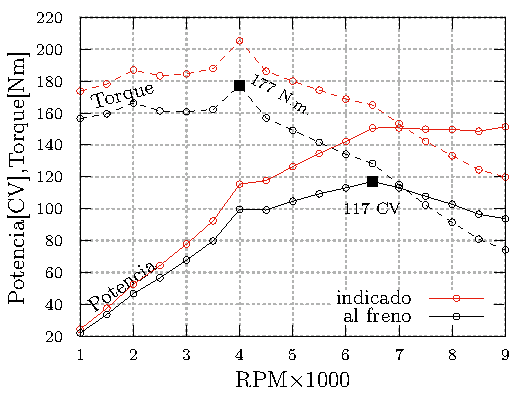
\includegraphics{/gnuplot/segunda_iter_pot.pdf}
\caption{Segunda Iteración} \label{fig:primer_op}
\end{figure}


El motor tiene una potencia máxima de 117 CV a las 6500 RPM y un par máximo de
177Nm a 4000 RPM, este coincide con el máximo de rendimiento volumétrico de
$\sim 0.845$
%
En la figura~\ref{fig:PoTi_segunda_op} se nota los efectos del coeficiente de descarga
en la simiulación del motor, el máximo

\begin{figure}
  \begin{center}
  \begin{tikzpicture}
    \begin{axis}[
      xlabel=Velocidad del motor [RPM],
      ylabel={$P_{i}[HP],T_{i}[N.m.]$},
      legend pos=south east,
      grid=both,
      ]
      \addplot[mark=o,solid,red] table [x=RPM,y=PotNet]{data/segundo_rend_vol.dat} ;
      \addplot[mark=o,solid,black] table [x=RPM,y=TorqNet]{data/segundo_rend_vol.dat} ;
      \addplot[mark=o,dashed,red] table [x=RPM,y=PotNet]{data/primer_rend_vol.dat} ;
      \addplot[mark=o,dashed,black] table [x=RPM,y=TorqNet]{data/primer_rend_vol.dat} ;
      \legend{$\dot{W}_{freno,2}$ , $T_{freno,2}$, $\dot{P}_{freno,1}$, $T_{freno,1}$}
    \end{axis}
  \end{tikzpicture}
  \end{center}
  \caption{Torque y Potencia de Segunda Iteración} \label{fig:PoTi_segunda_op}
\end{figure}
